\documentclass{article}
\usepackage[preprint,nonatbib]{neurips_2026}
\usepackage{fontspec}
\setmainfont{Times New Roman}
\setsansfont{Arial}
\setmonofont{Menlo}[Scale=0.82]
\newfontfamily\kyrgyz{Arial}
\usepackage{amsmath,amssymb,booktabs,graphicx,tabularx,array}
\usepackage[table]{xcolor}
\usepackage{microtype}
\usepackage{enumitem}
\usepackage{url}
\usepackage[colorlinks=true,linkcolor=teal!60!black,citecolor=teal!60!black,urlcolor=teal!60!black]{hyperref}
\hypersetup{pdftitle={Training Tiny Manas: A Small Language Model for a Kyrgyz Epic},pdfauthor={Nikita Nosov},pdfsubject={A retrospective empirical study of small-model training and optimization on Apple Silicon},pdfkeywords={Tiny Manas, Kyrgyz, language model, MPS, RoPE, ablation, reproducibility}}
\graphicspath{{figures/}}
\setlength{\emergencystretch}{1.5em}
\raggedbottom
\clubpenalty=10000
\widowpenalty=10000
\displaywidowpenalty=10000
\brokenpenalty=10000
\makeatletter\setlength{\@fptop}{0pt}\makeatother
\setlist{nosep,leftmargin=*}
\newcommand{\model}{Tiny Manas}
\newcommand{\code}[1]{\texttt{#1}}
\newcommand{\tabnote}[1]{\par\smallskip{\footnotesize #1}\par}
\title{Training Tiny Manas:\\A Small Language Model for a Kyrgyz Epic}
\author{Nikita Nosov\\\url{https://nik1t7n.com}\\\small Technical report · September 5, 2026}
\date{}

\begin{document}
\maketitle

\begin{abstract}
I trained Tiny Manas from scratch on the Kyrgyz epic \emph{Manas} to study small language models on a personal computer. The original corpus contains 465,069 tokens, encoded by a frozen 32,768-entry byte pair encoding (BPE) tokenizer. This report covers correctness checks, capacity and context comparisons, eleven optimization investigations, and a later data/evaluation/context/precision follow-up. On an Apple M5 with 16 GB of unified memory, increasing capacity improved prediction, and bfloat16 (BF16) reduced paired training-loop time by 20.58\%. Rotary position embeddings (RoPE) reduced original validation perplexity from 77.15 to 61.30. A subsequent corpus expansion supplied 343,402 additional training tokens and separate book-level holdouts. At a matched 3,000-update budget, it greatly improved the new-book score but worsened familiar-source loss by 0.045736 nats, exceeding the prespecified tolerance. A post-hoc partition exposed a substantial formatting contribution to that gain. The RoPE context-512 arm stopped at 1,500 updates without a consistent primary-score advantage; its full-budget outcome remains unknown. BF16 inference preserved prediction closely but made short generation 18.73\% slower. I therefore retained the 26,779,392-parameter RoPE model with context 256 and FP32 cached inference. The later report-only evaluation shows weak transfer to line-preserved texts from other sources. These single-seed findings describe the measured corpora, implementation, and budgets. The model has limited narrative coherence and is unsuitable as a general Kyrgyz assistant.
\end{abstract}

\section{Introduction}
I had used AI systems extensively before I could explain, line by line, how their weights learned to predict text. Tiny Manas became my first concrete milestone in closing that gap. Small Shakespeare models are a familiar educational starting point; I wanted the analogous experiment to begin with a text from my own linguistic context: \emph{Manas}.

My initial question was narrow: can I build the complete path from a real corpus to useful next-token predictions on my own computer? Once that path worked, a second question became more interesting: which common optimization and architecture choices help this small model on Apple Silicon? A technique can be valuable in a large CUDA workload and still be slower, unnecessary, or harmful under a different implementation and budget.

I therefore treated each change as a question rather than an upgrade by definition. The sequence also exposed a flaw in my own selection procedure. I initially stopped RoPE after a modest timing regression, without measuring its learned prediction quality. Reopening that decision produced the strongest architectural improvement in this study. The timing probe had answered a different question from the one needed to select an architecture.

This is a retrospective, artifact-backed technical report. The model design uses established Transformer components; I do not propose a new architecture or claim state-of-the-art Kyrgyz performance. My contribution is an end-to-end implementation record, controlled local comparisons, retained negative results, and an explicit account of where the measurements support a conclusion and where they do not. The implementation, configurations, and experiment reports are maintained in \href{https://github.com/nik1t7n/tiny-manas}{the Tiny Manas repository}. I retain the records' E identifiers for initial experiments and O identifiers for optimization studies.

\section{Data and tokenization}
\label{sec:data}
\subsection{Two corpora with different jobs}
A tokenizer learns how to divide text into reusable pieces. A language model learns how those pieces follow one another. These are separate training problems, and their data budgets must not be conflated.

Before this project, I built a Kyrgyz byte-level BPE tokenizer. The version used here was trained through the tokenizer project's original corpus-v1 pipeline, not its later bilingual experiments. That corpus contains 188,208 documents and 524,284,895 UTF-8 bytes. Its training split contains 186,360 documents and 518,527,574 bytes; its validation split contains 1,848 documents and 5,757,321 bytes. Table~\ref{tab:tokenizer-corpus} records the complete selected mixture before that split.

\begin{table}[ht]
\caption{The earlier tokenizer corpus. These texts trained the tokenizer, not Tiny Manas's language-model weights. Source shares refer to bytes.}
\label{tab:tokenizer-corpus}
\centering\small
\begin{tabular}{lrrr}
\toprule Source & Documents & UTF-8 bytes & Share \\
\midrule
FineWeb2, \code{kir\_Cyrl} & 52,374 & 236,088,121 & 45.03\% \\
Kyrgyz Wikipedia & 74,322 & 136,746,810 & 26.08\% \\
Kyrgyz News Corpus & 60,771 & 131,071,033 & 25.00\% \\
Manas-UdS & 741 & 20,378,931 & 3.89\% \\
\midrule Total & 188,208 & 524,284,895 & 100\% \\
\bottomrule
\end{tabular}
\end{table}

The tokenizer corpus pipeline used normalized-text hashing for exact duplicates and verified word-shingle similarity for near duplicates. It removed 18,777 near-duplicate documents before final selection. These operations belong to the earlier tokenizer build; I did not rerun them or claim a newly deduplicated language-model benchmark. Manas material is present in that tokenizer corpus. Consequently, a passage held out from LM weight training is \emph{not} necessarily unseen by the tokenizer-learning process.

The frozen tokenizer has 256 base-byte entries and 32,512 additional BPE entries, for 32,768 total. It uses no special/chat tokens and no text normalization. Rare text remains representable through byte pieces. Its complete artifact is pinned by commit and SHA-256 in the repository's provenance records; I did not silently replace it with the tokenizer repository's newer default. The full cleaned epic uses 9,593 distinct vocabulary IDs, but the model still predicts over all 32,768 entries.

\subsection{The actual language-model corpus}
For the original LM experiments I selected only document \code{Manas01} from the Manas-UdS archive \code{kyrgyz\_2022\_10\_03.zip}. Source metadata identifies \emph{Manas}, Sayakbai Karalaev, and a 2010 edition. The parser reads the surface-token column of the VRT source, reconstructs sentences, repairs punctuation spacing, and joins sentences with spaces. Thus the processed representation does not preserve the original page or verse-line layout.

I removed the introductory material at one verified, unique epic-start heading. This excluded 30,877 leading characters. The resulting text contains 1,794,194 characters, 3,249,652 UTF-8 bytes, and 465,069 tokenizer tokens. Exact encode/decode round trips were required for both the reconstructed document and the selected epic.

\begin{table}[ht]
\caption{Chronological LM splits. The tokenizer is fixed; token IDs are stored as little-endian unsigned 16-bit integers.}
\label{tab:splits}\centering\small
\begin{tabular}{lrrl}
\toprule Split & Tokens & Decoded UTF-8 bytes & Role \\
\midrule
Training & 418,562 & 2,924,452 & Weight updates \\
Validation & 23,253 & 164,489 & Selection and comparisons \\
Test & 23,254 & 160,711 & Post-selection reporting \\
\bottomrule
\end{tabular}
\end{table}

Table~\ref{tab:splits} shows the full experiment's 90/5/5 chronological split, not randomly shuffled fragments across splits. Training windows stay inside the training prefix. The 10,000-token pilot instead uses the first 10,000 tokens, split into 9,000 training and 1,000 validation tokens, with no separate test set. Pilot losses and full-corpus losses therefore describe different held-out text and are not directly comparable.

The source records describe Manas-UdS as CC BY-NC-SA 4.0. Other tokenizer sources have their own terms, including non-commercial components. I preserve provenance and do not redistribute these text payloads in the code repository. This report does not grant commercial rights to the corpus or resolve the legal status of trained weights. Exact locks and source-specific notices are retained rather than replaced by one blanket dataset license.

\subsection{O14: an additional corpus and book-level holdouts}
The September 5 follow-up admits three Orozbakov volumes for training and separates two other books before inspecting model scores (Table~\ref{tab:expanded-data}). I obtained the editions from the Bizdin collection~\cite{bizdin} and confirmed permission to use them for this student research. This records the research authorization; it does not assert an independently verified Creative Commons license for every scanned edition. The public repository contains the extraction code and source hashes, not the books or their complete transcriptions.

\begin{table}[ht]
\caption{O14 source groups, fixed before O15 training. The original training prefix is unchanged. Page numbers refer to the downloaded PDF, not printed page labels.}
\label{tab:expanded-data}\centering\small
\begin{tabular}{llrr}
\toprule Source & Role & PDF pages & Tokens \\
\midrule
Karalaev, original prefix & Train & VRT source & 418,562 \\
Orozbakov, book 2 & Train & 17--380 & 110,252 \\
Orozbakov, book 3 & Train & 10--299 & 91,367 \\
Orozbakov, book 5 & Train & 18--561 & 141,783 \\
Orozbakov, book 4 & Validation & 16--332 & 99,630 \\
Jusup Mamay & Test & 29--1040 & 408,359 \\
\bottomrule
\end{tabular}
\end{table}

Ordinary PDF extraction split some words into letters and mixed verse with scholarly notes. I instead used word coordinates to rejoin fragments, exclude smaller-type editorial apparatus, and remove counters and watermarks. Contents pages and section boundaries determined the verse ranges; spot checks compared extracted text with rendered pages. The extraction preserves verse newlines and does not generate replacement text or guess OCR spelling corrections. Residual recognition errors remain. Three other downloaded volumes were excluded because their dense apparatus, multi-column layout, or glyph errors required additional work.

All admitted texts pass exact encode/decode and UTF-8 byte-accounting checks with the frozen tokenizer; no replacement characters occur. Screening case-folded exact 32-word spans against the new and historical holdouts, then earlier training sources, found no spans to remove. The screening cannot rule out near-duplicates, short formulas, or OCR-obscured copies. Orozbakov volumes belong to one related academic edition. Mamay supplies a different narrator for LM evaluation, but historical tokenizer exposure is not ruled out.

The expanded training pool contains 761,964 tokens, including 343,402 new tokens. Half of each expanded-arm microbatch comes from the original source and half from the new volumes, sampled in proportion to eligible window starts. Windows cannot cross a source boundary. This treatment jointly changes textual coverage, source weighting, and line formatting; it is not an isolated estimate of narrator diversity.

The primary selection score uses 256 evenly spaced, nonoverlapping spans of up to 128 target tokens across book 4. A 512-token prefix supplies context only. The familiar-domain control scores the complete original validation suffix after the same prefix exclusion. Contexts 256 and 512 use identical target positions: a full span gives each target respectively 129--256 or 385--512 preceding tokens. Summed negative log likelihood is divided by the exact number of targets for token loss, and by their decoded UTF-8 byte count and $\log 2$ for bits per byte. Whole-book and Mamay scores are report-only after selection. These definitions differ from the earlier random-window and O05 protocols.

\section{Model: a small pre-normalized decoder}
\label{sec:model}
The main computational object is a vector for each token position. Attention lets that position collect information from earlier positions; a feed-forward network (FFN) transforms the collected features. Residual additions preserve the incoming representation and add the new message. Eight blocks refine the representation before a vocabulary projection produces next-token scores. Figure~\ref{fig:architecture} shows the current model.

Tiny Manas follows the decoder-only, pre-normalized design associated with GPT-2~\cite{gpt2}, using the causal attention mechanism introduced by Vaswani et al.~\cite{attention}. There is no encoder and no cross-attention. I used nanoGPT~\cite{nanogpt} as an implementation reference for a compact decoder, tied embeddings, initialization, and optimizer grouping, while maintaining a separate data, training, experiment, and serving implementation.

\begin{figure}[ht]
\centering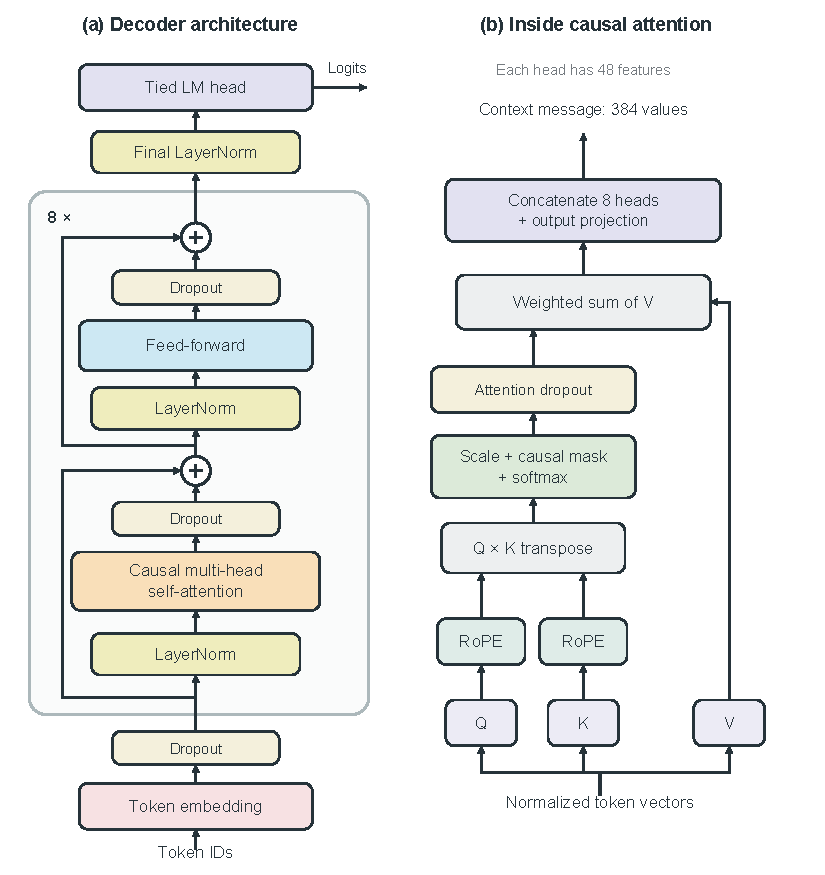
\includegraphics[width=\linewidth]{architecture.pdf}
\caption{The current native model, after the RoPE reevaluation. (a) Each residual route starts \emph{before} normalization and returns after its sublayer's dropout. (b) Query and key vectors receive rotary position transformations; value vectors do not. Attention-weight dropout is distinct from the output dropout in (a). All dropout is disabled for evaluation and generation. The diagram depicts the implemented decoder.}
\label{fig:architecture}
\end{figure}

\subsection{From token IDs to context-dependent vectors}
Let $L=8$ be the number of blocks, $B$ the microbatch size, $T\leq256$ its sequence length, $C=384$ the residual width, $H=8$ the number of heads, and $d=C/H=48$ the width of one head. For vocabulary $\mathcal{V}$, with $|\mathcal{V}|=32768$, a lookup into $E\in\mathbb{R}^{32768\times384}$ maps IDs to $X\in\mathbb{R}^{B\times T\times384}$. The original model added a learned position table $P\in\mathbb{R}^{256\times384}$ before embedding dropout. The current model removes $P$ and places positional information inside attention through RoPE.

Using row-vector notation, each block first normalizes its input $Z=\mathrm{LN}(X)$ and computes
\begin{equation}
 Q=ZW_Q+b_Q,\qquad K=ZW_K+b_K,\qquad V=ZW_V+b_V.
\end{equation}
The implementation packs these projections into one linear operation and reshapes each output into $(B,H,T,d)$. These are computed activations, not permanent query/key/value tables for vocabulary items. Each head uses all 384 input features to create its own 48-feature representation.

For the rotation below, individual query and key vectors use column notation. Pair $j$ at position $m$ is rotated by angle $m\omega_j$, where $\omega_j=10000^{-2j/d}$ and $j=0,\ldots,d/2-1$:
\begin{equation}
\begin{pmatrix}\widetilde u_{2j}\\\widetilde u_{2j+1}\end{pmatrix}
=\begin{pmatrix}\cos(m\omega_j)&-\sin(m\omega_j)\\\sin(m\omega_j)&\cos(m\omega_j)\end{pmatrix}
\begin{pmatrix}u_{2j}\\u_{2j+1}\end{pmatrix},\qquad u\in\{q,k\}.
\label{eq:rope}
\end{equation}
Writing the full block-diagonal rotation as $R_m$, the query--key dot product satisfies $(R_mq)^\top(R_nk)=q^\top R_{n-m}k$. This is the positional mechanism studied by Su et al.~\cite{rope}. My implementation uses adjacent pairs, precomputed non-trainable sine/cosine buffers, and 32-bit floating-point (FP32) rotation arithmetic before restoring the incoming query/key dtype. This description does not imply that the trained model supports longer contexts: the configured and tested limit remains 256.

Within each head the context message is
\begin{equation}
 A=\mathrm{softmax}\!\left(\frac{\widetilde Q\widetilde K^\top}{\sqrt{48}}+M\right),
 \qquad U=\mathcal{D}_{0.2}(A)V,\qquad
 M_{ij}=\begin{cases}0&j\leq i,\\-\infty&j>i.\end{cases}
\label{eq:attention}
\end{equation}
The mask prevents a training position from reading its future answer. Softmax operates over keys, giving each query a distribution over allowed positions \emph{before} dropout. Head outputs are concatenated into 384 features and projected by $W_O$. The native implementation calls scaled dot-product attention through Apple's Metal Performance Shaders (MPS) backend; this does not by itself establish that a particular FlashAttention kernel ran on MPS.

\subsection{Normalization, feature transformation, and residual paths}
LayerNorm~\cite{layernorm} independently normalizes the $C$ features of each token, with learned gain and bias:
\begin{equation}
\mathrm{LN}(x)=\gamma\odot\frac{x-\mu(x)}{\sqrt{\sigma^2(x)+10^{-5}}}+\beta.
\end{equation}
Here $\mu(x)$ and $\sigma^2(x)$ are the mean and variance across the token's $C$ features; $\odot$ denotes elementwise multiplication. The two residual operations are
\begin{align}
 X'&=X+\mathcal{D}_{0.2}\!\left(\mathrm{Concat}(U_1,\ldots,U_8)W_O+b_O\right),\\
 X^{\mathrm{next}}&=X'+\mathcal{D}_{0.2}\!\left(\mathrm{GELU}(\mathrm{LN}(X')W_1+b_1)W_2+b_2\right).
\end{align}
The FFN expands 384 features to 1,536 and projects back to 384. It operates at each position with the same weights; it does not read other positions directly. I retain the Gaussian error linear unit (GELU) FFN because the parameter-matched SwiGLU experiment did not improve this recipe.

Dropout~\cite{dropout} is present at embeddings, attention weights, attention output, and FFN output. Here $p=0.2$ denotes the \emph{drop probability}, unlike the retention-probability notation in parts of the original paper. During training, $\mathcal{D}_p(z)=m\odot z/(1-p)$ with independent $m_i\sim\mathrm{Bernoulli}(1-p)$; during evaluation it is the identity. The scaling preserves the expectation, not the exact magnitude of every sampled vector. After attention dropout, a realized attention row need not sum to one.

A final LayerNorm precedes the bias-free LM head. Its weights are tied to $E$, so logits are $\mathrm{LN}(X^{(8)})E^\top$, where $X^{(8)}$ is the output of the eighth block. Tying prevents a second 12.58M-parameter vocabulary matrix.

\section{Training and evaluation protocol}
\label{sec:protocol}
\subsection{What the model is trained to do}
For a sampled slice $(s_0,\ldots,s_T)$, the input is $(s_0,\ldots,s_{T-1})$ and the target is $(s_1,\ldots,s_T)$. Every input position contributes one next-token prediction. With model parameters $\theta$ and natural logarithms, the mean negative log-likelihood is
\begin{equation}
\mathcal{L}(\theta)=-\frac{1}{BT}\sum_{b=1}^{B}\sum_{t=0}^{T-1}
\log p_\theta(s_{b,t+1}\mid s_{b,0:t}).
\label{eq:loss}
\end{equation}
The implementation passes logits directly to full-vocabulary cross-entropy. It does not select a sampled next token during training. Backpropagation computes parameter gradients; AdamW~\cite{adamw} then updates the parameters. Ordinary matrix parameters receive weight decay, while one-dimensional biases and normalization parameters do not.

Table~\ref{tab:recipe} summarizes the main training settings. For the 27M comparisons, $B=8$ and two microbatches accumulate before one optimizer update. Each microbatch loss is divided by two before backward, yielding $8\times256\times2=4,096$ target positions per update. The 3,000-update budget exposes the model to 12,288,000 sampled targets: roughly 29.36 times the number of training tokens, \emph{not} 12.3 million distinct tokens or exactly 29.36 sequential epochs.

\begin{table}[ht]
\caption{Main training recipe. One controlled variable changes per principal comparison unless the report explicitly identifies a different protocol.}
\label{tab:recipe}\centering\small
\begin{tabularx}{\linewidth}{lX}
\toprule Setting & Value \\
\midrule
Hardware / backend & Apple M5, 16 GB unified memory; PyTorch 2.13.0; MPS backend, with no CPU fallback \\
Initialization / sampling seeds & 1337 / 1338 for training windows \\
Optimizer & AdamW, $\beta_1=0.9$, $\beta_2=0.95$, weight decay $0.1$ \\
Learning rate & 100-step linear warmup to $3\times10^{-4}$; cosine decay toward $3\times10^{-5}$ over the 3,000-step recipe \\
Gradient norm clipping & Global norm capped at 1.0 after accumulation \\
Initialization & Normal $\sigma=0.02$; zero linear biases; residual projections use $0.02/\sqrt{2L}$ \\
Precision & Initially FP32; BF16 autocast accepted for training; evaluation and inference FP32 \\
Checkpoint selection & Lowest scheduled validation loss; normally 30 batches every 100 updates \\
Quality evaluation & 100 additional random batches, FP32; seed 1837 \\
\bottomrule
\end{tabularx}
\end{table}

The model's parameters and AdamW states remain FP32 under mixed precision; BF16 is not a conversion of the entire training state. The generic code still supports FP32 for old experiments. The original full-corpus runs had patience-based early stopping, but all three reached 3,000 updates. Later controlled full comparisons disabled that early stop so both arms received the same budget. The pilot and diagnostic overfit run have their own smaller configurations.

\subsection{Validation protocols and evaluation metrics}
\label{sec:metrics}
\textbf{Scheduled validation} selects a checkpoint using 30 random batches. \textbf{Additional validation} evaluates that checkpoint on 100 batches with a separate sampler seed: 204,800 target positions at $B=8,T=256$. This is a larger resampling of the \emph{same} validation suffix, not a new independent dataset. Repeated windows and overlapping contexts mean these target positions are not 204,800 independent observations.

\textbf{Perplexity (PPL)} is $\exp(\mathcal{L})$; lower is better for the same tokenization and evaluation protocol. A 0.02-nat loss reduction corresponds to about a 1.98\% perplexity reduction. Neither perplexity nor next-token top-1 accuracy measures factuality, instruction following, or narrative coherence.

For comparisons across tokenizers, the unit of prediction changes. I therefore report bits per byte (BPB) using exact-byte scoring:
\begin{equation}
\mathrm{BPB}=\frac{\sum_{i\in\mathcal{S}}-\log p_\theta(s_i\mid\mathrm{context}_i)}{\ln(2)\,N_{\mathrm{UTF8}}}.
\label{eq:bpb}
\end{equation}
Here $\mathcal{S}$ contains the scored target-token positions and $N_{\mathrm{UTF8}}$ counts their original UTF-8 bytes. All candidates score the same target bytes, each target once, using at most 256 context tokens and 128 scored targets per evaluation window. A common 129-byte validation prefix supplies initial context, leaving 164,360 scored bytes. This is different from the historical approximation that multiplied random-batch mean token loss by the whole split's average tokens per byte. I do not pool those two BPB definitions in a table. The final test's stored byte-normalized field is still the historical approximation; the main test claims use loss and perplexity.

Test reporting occurs after each relevant selection phase, never inside the staged RoPE/RMSNorm rules. However, the same chronological suffix was already examined in the earlier capacity study. It is not a newly sequestered, never-before-seen final benchmark. The entire research sequence is adaptive and single-seed; I do not report statistical significance or seed-level error bars that were never measured.

\section{From a broken measurement to a working language model}
\label{sec:initial}
\subsection{E0--E2: validate the loop before scaling it}
The initial execution check on corpus data produced logits of shape $(4,64,32768)$ and loss 10.4317, near the uniform-vocabulary value $\ln(32768)=10.3972$. The backward pass produced finite gradients. In a bounded causal check, changing future tokens left the inspected prefix logits unchanged. This established a usable execution path, not learned language ability.

I then asked the smallest useful training question: can the model intentionally memorize one real batch? The first attempt appeared to fail. In fact, optimization loss had already fallen from 10.4385 to 0.0280 by update 100, while the periodic ``training'' evaluator reported an unrelated high loss. It was drawing a different fixed batch with another seed. The stopping rule therefore evaluated a batch the model had not been trained to memorize.

After correcting the sampler identity, the 4.60M-parameter, two-block model reached loss 0.02673 and 100\% top-1/top-5 accuracy on its fixed batch at update 100. Training stopped after 25,600 target positions and 1.89 seconds of measured loop time. This is deliberate memorization, not a validation success. The invalid first summary remains in the experiment record instead of being silently replaced.

The 8.10M-parameter pilot used four blocks, width 192, context 128, and dropout 0.2 on the first 10,000 tokens. It made useful initial progress, then memorized the small training prefix. Best scheduled validation loss was 7.3231 at update 200; by update 1,000, training loss had fallen to 0.1235 while validation loss had climbed to 10.4687. Eight unsuccessful evaluations triggered early stopping. A separate 50-batch check of the best checkpoint gave loss 7.3369. Better-looking snippets from the final overfit checkpoint did not override the held-out result.

\begin{figure}[ht]
\centering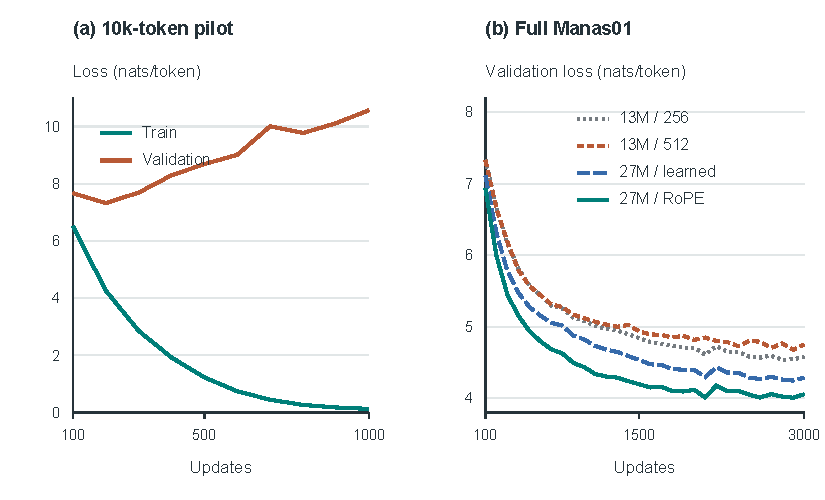
\includegraphics[width=\linewidth]{learning-curves.pdf}
\caption{Observed scheduled evaluation curves, extracted from saved metrics. (a) The pilot's training and validation losses separate sharply; its validation text differs from the full-corpus study. (b) Full-Manas01 comparisons show why capacity and context need separate evaluation. The RoPE line comes from the later controlled study, not the original FP32 capacity run. Lines connect recorded checkpoints; no smoothing, synthetic points, or uncertainty bands are added.}
\label{fig:learning}
\end{figure}

\subsection{E3--E5: corpus size, context length, and model capacity}
Moving to the complete epic and the planned 13.2M configuration produced a functioning Manas-style generator. This step changed both data and model size, so it is not an isolated causal estimate of the benefit of more data. It established a baseline for the next controlled comparisons (Table~\ref{tab:original}). Figure~\ref{fig:learning} shows the recorded learning curves.

\begin{table}[ht]
\caption{Original full-corpus experiments, all FP32 with 3,000 updates and 12,288,000 sampled targets. Losses use the additional held-out evaluation, not the lower scheduled checkpoint-selection score.}
\label{tab:original}\centering\small
\begin{tabular}{lrrrrr}
\toprule Model / context & Parameters & Val. loss & Val. PPL & Test PPL & Loop min. \\
\midrule
13M / 256 & 13,193,216 & 4.6384 & 103.38 & 151.42 & 15.10 \\
13M / 512 & 13,258,752 & 4.7268 & 112.94 & 171.85 & 17.22 \\
27M / 256 & 26,877,696 & 4.3457 & 77.15 & 116.45 & 24.45 \\
\bottomrule
\end{tabular}
\end{table}

Doubling context from 256 to 512 retained width 256 and six layers. I halved the microbatch from eight to four, keeping two accumulation steps and 4,096 targets per update. The longer position table added 65,536 parameters. Validation and test prediction both worsened, and target throughput fell from 13,565 to 11,894 per second. The longer window also means fewer independent sampled windows per update; this is a fixed-target-budget comparison, not a universal claim that long context is harmful.

I next retained context 256 and increased depth to eight and width to 384. Test perplexity fell from 151.42 to 116.45, and validation perplexity from 103.38 to 77.15, at a throughput cost: 8,378 targets per second. The original 27M model was the best tested full-corpus configuration at this stage. Its best checkpoint was update 2,900, not the final update. That checkpoint and the original source checkout were frozen before optimization.

These measurements answered the local engineering question: additional capacity helped this recipe more than a longer context did. They do not identify a scaling law or an optimal parameter count. Only two capacity settings and one longer-context alternative were evaluated.

\section{Optimization study: speed, memory, and correctness}
\label{sec:systems}
I separated equivalent execution changes from architectural changes. Table~\ref{tab:systems} summarizes the systems experiments. An equivalent execution path must preserve the intended computation before a timing result matters. An architectural change can alter learned quality, so shape correctness or a fast forward pass is not enough to accept it.

\begin{table}[ht]
\caption{Systems experiments on the original 27M architecture. Timing definitions differ by row and are not additive. Allocation samples are not total-process peaks.}
\label{tab:systems}\centering\small
\begin{tabularx}{\linewidth}{lXXl}
\toprule Change & Measurement & Observed result & Decision \\
\midrule
O01: last-position logits & FP32 forward, $B=1,T=256$ & 7.307 to 5.894 ms; output 32 MiB to 128 KiB & Adopt \\
O02: BF16 & Matched full training-loop time & 1,548.04 to 1,229.41 s; val. $+0.0000464$ nats & Adopt \\
O03: compile & Warm paired update median & 0.32365 to 0.33343 s after correctness repair & Reject \\
O04: recompute & Update median / live allocation samples & $+30.63\%$ latency; $-38.46\%$ allocation & Optional \\
O09: KV cache & 32-token prompt + 64 generated & 0.19675 to 0.17011 s; 1.157$\times$ & Adopt \\
O11: fused loss & Conditional bottleneck assessment & No blocking logit-memory constraint measured & Not run \\
\bottomrule
\end{tabularx}
\end{table}

\subsection{O01--O02: avoid discarded logits; use BF16 selectively}
During generation, earlier-position vocabulary scores are discarded. Slicing hidden states \emph{before} the LM head reduces output storage from $BT|\mathcal{V}|$ values to $B|\mathcal{V}|$ while leaving training unchanged. Numerical comparisons and greedy continuations passed on real prompts, including context overflow. At $T=1$ there is nothing to save and the microbenchmark was slightly slower; I do not claim a context-independent speedup.

BF16 was first tested for 100 paired updates, then for two fresh, matched 3,000-update runs. Forward autocast changed, but FP32 evaluation, initialization, training windows, dropout rate, and optimizer recipe did not. The full-loop time fell by 20.58\%, while additional validation losses were 4.345733 (FP32) and 4.345779 (BF16). The improvement concerns local throughput; the measured prediction quality was nearly unchanged.

The memory result depends on where it was sampled. The short probe's within-step live allocation fell only 2.1\%; full-run after-update samples fell 33.83\%, while driver allocation rose 0.36\%. I retain those definitions rather than claiming BF16 halved training memory. The 20 saved outputs from each full run were reviewed; their general failure modes remained similar, although individual continuations changed substantially.

\subsection{O03--O04: correctness failures that a loss scalar missed}
The first compiled MPS attempt had a small loss difference but a relative gradient error of 1.33376. Inspection of individual parameter gradients localized the discrepancy to broadcasting the positional embedding lookup. A research-only rewrite explicitly indexed positions at shape $(B,T)$, reducing relative gradient error to 0.00651, within the BF16 gate. The corrected compiler route then ran 3.02\% slower over 30 post-warmup paired updates. The measured steady-state execution was slower, so this run offered no way to amortize the compilation cost. I retained eager execution. This result is specific to the installed backend, expression, and shapes.

Activation checkpointing~\cite{checkpoint} trades saved intermediates for recomputation during backward. The first MPS attempt reproduced the forward loss but not the gradients: relative error was 0.675827 because recomputation did not preserve the required MPS dropout state. Saving and restoring the device's random number generator (RNG) state reduced the corrected error to approximately $6.0\times10^{-9}$. Over 35 real updates per arm, excluding five warmup updates, sampled live allocation fell from 2,099,575,552 to 1,292,135,680 bytes, while median update time rose from 0.317603 to 0.414878 seconds.

The corrected option is integrated but disabled by default. The accepted small model already fits; spending roughly 31\% more update time for unused memory headroom would not serve this experiment. Neither this result nor the compile failure is evidence about every MPS version, CUDA, or combined compiled checkpointing.

\subsection{O11: fused-loss assessment}
At $B=8,T=256,|\mathcal{V}|=32768$, one BF16 logits tensor occupies 128 MiB; the FP32 equivalent occupies 256 MiB. That is substantial, but the observed model fit within the configured budget. I considered fused/chunked cross-entropy, including Cut Cross-Entropy~\cite{cce}, and did not implement a new loss kernel without a measured need. No fused-loss runtime result exists. A streamed full-vocabulary loss and optional backward approximations also require separate numerical claims; I do not label every implementation ``exact'' without qualification.

\section{O05: vocabulary size under an equal-text budget}
\label{sec:vocab}
A smaller vocabulary shrinks the tied embedding/head matrix, but makes the same text longer in tokens. Equal optimizer steps would then expose candidates to different amounts of original text. I used an equal-text experiment instead of treating per-token perplexity as comparable across vocabularies.

The earlier tokenizer project already contained nested BPE variants with 32,768, 16,384, and 8,192 entries (32k, 16k, and 8k below), trained on the same corpus with the same preprocessing. Their recorded artifacts and shard hashes were verified; no new tokenizer training was required. I preserved the original \emph{byte} boundaries of the train/validation/test text before retokenizing. Thirty complete passes over the same scored training bytes were used for each candidate, with learning rate scheduled by text exposure. A shared 126-byte training prefix remained unscored. Each arm processed 87,729,780 scored source bytes.

Non-overlapping training windows were shuffled per pass. Short final windows used ignored targets, not a new padding token, and accumulated losses were weighted by actual target counts. Shared Transformer tensors were initialized identically; matching embedding IDs inherited matching fresh rows. Depth, width, and 256-token context stayed fixed, but vocabulary capacity and the number of updates necessarily differed.

\begin{table}[ht]
\caption{Equal-text tokenizer comparison. ``Incumbent'' uses the earlier random-window recipe and serves as a deployment quality floor, not as the controlled tokenizer arm. All BPB values use the same 164,360 target bytes.}
\label{tab:vocab}\centering\small
\begin{tabular}{lrrrrr}
\toprule Model & Params (M) & Updates & Val. BPB & Bytes/s & Alloc. (GiB) \\
\midrule
32k incumbent & 26.878 & 3,000 & 0.87644 & --- & --- \\
32k equal-text & 26.878 & 3,090 & 0.92129 & 82,253 & 2.10 \\
16k equal-text & 20.586 & 3,420 & 0.91285 & 95,484 & 1.68 \\
8k equal-text & 17.441 & 3,840 & 0.91012 & 99,115 & 1.58 \\
\bottomrule
\end{tabular}
\tabnote{Bytes/s excludes scheduled validation, checkpoint writes, and generation audit. Allocation is a sampled live tensor quantity, not unified-memory occupancy.}
\end{table}

\begin{figure}[ht]
\centering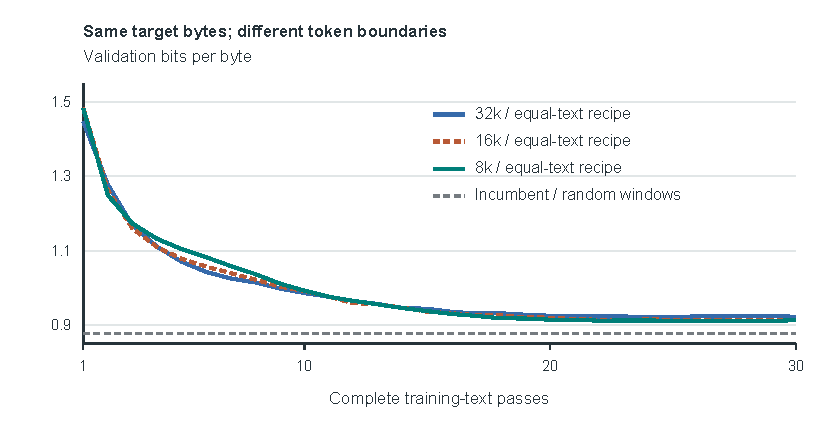
\includegraphics[width=\linewidth]{tokenizer-curves.pdf}
\caption{Recorded exact-byte validation curves. Smaller vocabularies slightly outperform the fresh 32k arm under the shared equal-text recipe, but none reaches the previously accepted model's quality. The dashed incumbent line is a checkpoint score, not a missing training trajectory.}
\label{fig:tokenizer}
\end{figure}

Table~\ref{tab:vocab} and Figure~\ref{fig:tokenizer} report the comparison. The 16k and 8k variants improved byte throughput by 16.09\% and 20.50\% over fresh 32k. They also improved BPB by 0.92\% and 1.21\% within that controlled recipe. However, their BPB remained 4.15\% and 3.84\% worse than the incumbent, failing the predeclared 1\% degradation ceiling. I kept the original 32k tokenizer and random-window training recipe.

The fresh 32k control itself was 5.12\% worse than the incumbent, so this result does not establish that 32k is the best vocabulary size. Sampling, schedule, and selection changed between those recipes. The controlled comparison supports a resource/quality tradeoff among vocabulary sizes; the separate incumbent floor prevents adopting a worse delivered model. It cannot identify which recipe change caused the control regression. Sixty candidate continuations were inspected, but equal generated-token budgets produced different byte lengths, limiting copying and repetition comparisons.

\section{Architectural alternatives and the quality-gate correction}
\label{sec:architecture-results}
\subsection{O06--O07: why I reopened RoPE and RMSNorm}
The initial numerical/cost gates accepted the mathematical implementations of RoPE and RMSNorm but stopped before full training: their measured updates were 12.27\% and 10.70\% slower. That was sufficient to reject a speed claim, not to reject a possible quality gain. I revised the policy and recorded a bounded quality follow-up protocol before continuing.

Candidates started from a saved \emph{fresh initializer}, not a trained checkpoint. The same 3,000-step learning-rate schedule remained in force during short prefixes of the run; I did not compress the schedule into a pilot and then extrapolate its results. A 100-update control calibration reproduced the archived BF16 trajectory closely: the largest checked train-point difference was 0.0001164 nats, and the validation difference was approximately 0.0000065. On the basis of this calibration, I reused the full historical control rather than repeat its training run.

Validation was checked every 100 updates. No quality pruning occurred before update 600. From update 900 onward, a candidate without a material improvement and without an improving relative gap could stop; a promising candidate had to pass the 1,500-update gate and then complete 3,000 updates. The practical gain floor was 0.02 nats, not a statistical confidence threshold. The repository's quality follow-up protocol records the rules. This is a small, predeclared staged allocation policy in the spirit of early resource allocation~\cite{hyperband}, not an implementation of Hyperband.

\begin{figure}[ht]
\centering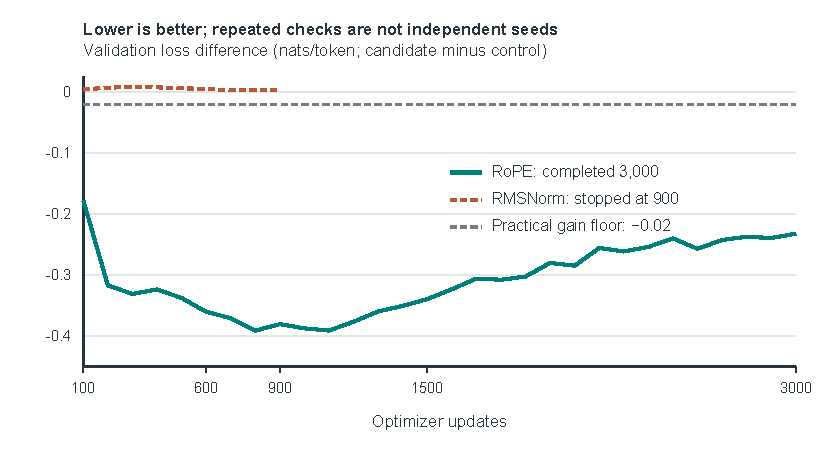
\includegraphics[width=\linewidth]{staged-quality.pdf}
\caption{Quality follow-up trajectories relative to the matched archived BF16 control. RoPE's persistent validation improvement met the rule for completing the full budget. RMSNorm remains close to the control and stops at 900 updates. The plotted points are correlated scheduled evaluations; their number does not replace multiple training seeds.}
\label{fig:staging}
\end{figure}

\subsection{RoPE: a full-budget improvement}
Figure~\ref{fig:staging} shows the staged comparison; Table~\ref{tab:rope} reports the selected checkpoints. RoPE's recent three-check mean loss advantage was already 0.34082 nats at update 600 and remained substantial at later gates. It completed 3,000 updates and selected update 2,900. The final additional-validation loss fell from 4.345779 to 4.115836: a 0.229944-nat reduction and a 20.54\% reduction in perplexity. Exact-byte BPB fell from 0.876442 to 0.827695. The 20-generation audit did not reveal a new class of collapse, although it did not establish better human-rated coherence.

\begin{table}[ht]
\caption{The accepted architecture change. Both models use the same 32k tokenizer, 256-token context, and 3,000-update BF16 recipe. Test scores were reported after selection. Generation metrics use 20 continuations per model (Section~\ref{sec:generation-audit}).}
\label{tab:rope}\centering\small
\begin{tabular}{lrr}
\toprule Measurement & Learned positions & RoPE \\
\midrule
Parameters & 26,877,696 & 26,779,392 \\
Additional validation loss & 4.345779 & 4.115836 \\
Additional validation perplexity & 77.152 & 61.303 \\
Exact-byte validation BPB & 0.876442 & 0.827695 \\
Test loss & 4.757561 & 4.531258 \\
Test perplexity & 116.461 & 92.875 \\
Mean repeated-trigram ratio & 4.097\% & 4.134\% \\
Maximum normalized matching span & 9 words & 11 words \\
\bottomrule
\end{tabular}
\end{table}

The follow-up cost probe measured 0.33221 seconds per classic update and 0.36506 for RoPE, a 9.89\% regression in that session. It does not erase the earlier 12.27\% measurement; shared-host conditions and short probes vary. RoPE's saved segments total 1,101.24 seconds of \emph{update-only} training time, excluding evaluation, checkpointing, and audits. Comparing that narrower total with the BF16 control's complete loop time would incorrectly turn a slower operation into a speedup.

I integrated the measured candidate into the native model, preserving initializer order so shared tensors match the research initializer. Native and research checkpoint logits matched exactly in the recorded CPU conversion check. Cache parity was also checked, including overflow. The accepted inference artifact contains 26,779,392 parameters; its post-selection test top-1 and top-5 accuracies are 31.70\% and 48.53\%. These are token-prediction accuracies, not reading-comprehension scores.

\subsection{RMSNorm: a budget stop, not a universal rejection}
RMSNorm~\cite{rmsnorm} rescales by root-mean-square magnitude without subtracting the mean. Its lower algebraic complexity did not produce faster updates in this implementation. In the reopened run, the last three validation deltas at updates 700, 800, and 900 were $+0.002686$, $+0.003778$, and $+0.003471$ nats. Their mean, $+0.003312$, was close to the LayerNorm control and did not cross the practical gain floor. Relative-gap improvement versus the preceding three checks was only 0.002947 nats.

The rule stopped RMSNorm at update 900, saving 2,100 remaining updates (70\% of its planned full budget). I retained LayerNorm. I did \emph{not} measure RMSNorm's 3,000-update performance, final generations, or test score. A late crossover remains possible; the result supports this resource-allocation decision, not a claim that RMSNorm cannot improve a differently tuned model.

\subsection{O08 and O10: SwiGLU and grouped-query attention}
SwiGLU~\cite{swiglu} replaces the GELU FFN with a gated product. To compare similar capacity, I used hidden width 1,024 rather than the GELU path's 1,536: three projection matrices replace two. Including biases, the candidate has 26,881,792 parameters, only 4,096 above the classic model. The controlled cost probe was 3.80\% slower with 8.82\% more sampled allocation. After all 3,000 updates, additional-validation loss was 4.427423, worse than GELU by 0.081643 nats. Mean repeated trigrams rose from 4.10\% to 6.95\%, with a worst sample of 52.78\%. I retained GELU. This full negative result is stronger than an early flat curve, but remains specific to the fixed recipe and single seed.

Grouped-query attention (GQA)~\cite{gqa} shares key/value projections among query heads. I converted the accepted learned-position multi-head attention (MHA) checkpoint by mean-pooling K/V weights and biases from each group of four heads, retaining eight query heads and two KV heads. This was a \emph{checkpoint adaptation} experiment, not training GQA from scratch. Both converted GQA and unchanged MHA received 150 updates, fresh AdamW states, identical windows, and a fixed learning rate of $3\times10^{-5}$.

Persistent FP32 cache storage fell from 6 to 1.5 MiB. Interleaved decode timing was 1.10\% slower, within the latency tolerance. Prediction did not recover sufficiently: GQA's final validation loss on the exact-byte windows was 4.497047 versus adapted MHA's 4.303030, a 0.194018-nat gap above the 0.05 ceiling. GQA's loss had improved from 5.074695 immediately after conversion, so adaptation helped, but not enough. I retained MHA. These results do not answer whether a longer adaptation, another grouping, or fresh GQA pretraining would succeed; none was run.

\section{O15--O16: data and context under fixed training budgets}
\label{sec:data-context}
\subsection{O15: a large new-book gain that did not pass promotion}
The additional corpus changed what the model saw, not its 26,779,392-parameter RoPE architecture. I trained a fresh old-data control and a fresh expanded-data arm from the same initial weights and seed, with BF16 training, FP32 evaluation, and the original 3,000-update learning-rate horizon. Each update consumed 4,096 targets. Both arms completed all 12,288,000 targets; the expanded arm passed its staged checks at 900, 1,200, and 1,500 updates. The measured training-loop subtotals were 1,151.57 and 1,111.20 seconds, excluding evaluation and checkpoint saves. Since these were sequential runs on a shared laptop, their difference is not a paired inference or hardware speed claim.

\begin{table}[ht]
\caption{O15 prediction on the frozen new evaluation targets. Book loss is the primary selection criterion; familiar loss is a separate safety check. These losses are not the earlier random-window scores.}
\label{tab:data-results}\centering\small
\begin{tabular}{lrrr}
\toprule Checkpoint & Update & Book loss & Familiar loss \\
\midrule
Deployed RoPE & Historical 2,900 & 11.84687 & 4.08818 \\
Old-data control, primary-selected & 100 & 9.89860 & 6.95710 \\
Old-data control, final & 3,000 & 11.96507 & 4.09131 \\
Expanded data, primary-selected/final & 3,000 & 4.20787 & 4.13392 \\
\bottomrule
\end{tabular}
\end{table}

The expanded model greatly reduced new-book loss (Table~\ref{tab:data-results}), but its familiar loss exceeded the deployed model by 0.045736 nats. That violated the prespecified +0.02 limit. It also exceeded the fresh control's final familiar loss by 0.042609. I therefore did not promote the new weights. No generation audit or test evaluation was run for this already disqualified candidate. The result describes the chosen mixture and target budget; it does not show that additional Manas data cannot help.

The control exposed a problem with relying on the primary score alone: its best book score occurred at update 100, when familiar prediction was still poor. More old-source training improved familiar loss while worsening the differently formatted book score. The separate deployed-model floor prevented an undertrained control from making promotion artificially easy.

I added a post-hoc diagnostic after observing this divergence, without changing the data, checkpoints, or selection rule. It reproduced the final score on the same 32,686 book targets and partitioned them into 4,976 newline-bearing targets and 27,710 other targets. Mean loss on the first group fell from 25.1006 to 0.9245; on the second it fell from 9.6063 to 4.7975. Their weighted contributions to the aggregate changed from 3.8212 to 0.1407 and from 8.1438 to 4.0671, respectively. Direct newline-target loss accounts for about 47\% of the reduction. Other targets also improve, but their input contexts contain line breaks too. This partition cannot attribute the remaining gain solely to new content or narrator diversity.

\subsection{O16: the longer-context pilot stopped at 1,500 updates}
Since O15 did not replace the selected dataset, O16 used the original training text and the completed fresh 256-context control. The candidate changed only context and microbatch geometry: $4\times512\times2$ instead of $8\times256\times2$, retaining 4,096 targets per update, shared initial weights, and the full learning-rate horizon. The book-primary criterion remained fixed despite its observed formatting sensitivity. Figure~\ref{fig:data-context} shows both data and context trajectories.

The recent three-check mean primary deltas were -0.042100 at update 900 and -0.090285 at 1,200, permitting continuation. At 1,500 the last three deltas were +0.112277, -0.509526, and +0.411511; their mean was +0.004754. They failed the -0.02 effect floor and consistency requirement. I stopped the arm after 6,144,000 targets and 736.80 seconds of measured training-loop time, leaving half its maximum update budget unspent.

At that stopping point, book loss was 12.004335 using context 512 and 11.954920 using common context 256. The 256-trained control scored 11.592824. Familiar loss, measured at context 256 for both, was 4.236962 versus 4.224035. These are pilot results, not a completed trained-model comparison. No generation audit, native promotion, or test evaluation was run for the stopped arm. The result does not establish that a full-budget RoPE context-512 run would be worse.

\begin{figure}[ht]
\centering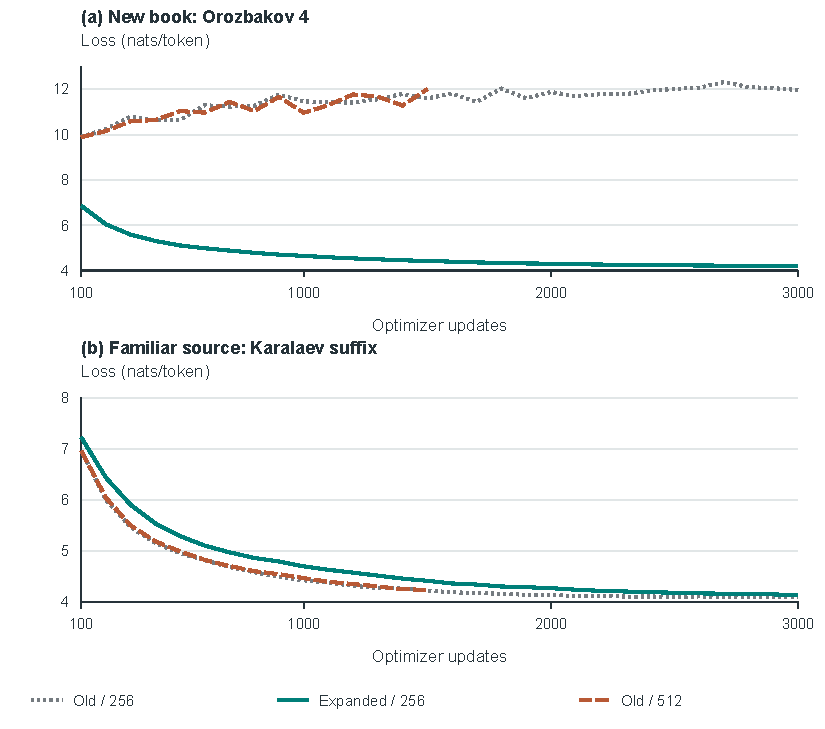
\includegraphics[width=\linewidth]{data-context-followup.pdf}
\caption{Observed O15/O16 curves, without smoothing or extrapolation. The primary score uses a line-preserved Orozbakov book; familiar validation uses the original flattened source. The expanded-data model improves the first score but fails the familiar-domain promotion floor. The original-data context-512 arm stops at 1,500; the two context-256 arms complete 3,000 updates. Repeated checks are not independent seeds.}
\label{fig:data-context}
\end{figure}

\subsection{Report-only evaluation after retaining the incumbent}
The four follow-up experiments did not justify new production weights or inference precision. After closing selection, I scored the unchanged export on every retained target in the full book and test remainders (Table~\ref{tab:book-test}). Each split contributes a 512-token context-only prefix; targets then appear once under the fixed 128-target stride. The high external-book losses expose weak transfer to these line-preserved, partly OCR-derived sources. They are not test results for the rejected expanded-data model, which was never scored on the protected Mamay test.

\begin{table}[ht]
\caption{The retained RoPE/256/FP32 checkpoint after selection. These whole-remainder scores have exact target and byte denominators. Cross-corpus score differences include text and formatting differences.}
\label{tab:book-test}\centering\small
\begin{tabular}{lrrrr}
\toprule Source & Targets & Scored bytes & Loss & Bits/byte \\
\midrule
Orozbakov 4, validation & 99,118 & 611,514 & 11.842740 & 2.769318 \\
Mamay, held-out test & 407,847 & 2,060,821 & 12.370524 & 3.531991 \\
Original test suffix & 22,742 & 156,951 & 4.534839 & 0.947984 \\
\bottomrule
\end{tabular}
\end{table}

Original-test perplexity is 93.21 under this protocol, compared with 92.88 under the older 100-random-batch protocol. The weights did not change; the evaluations use different target/context definitions. Across O15/O16, the three new training arms consumed 30,720,000 targets and 2,999.58 seconds in their training-loop subtotals. Source preparation, evaluation, and checkpoint saving are outside that subtotal. The final selected checkpoint did not require another training or inference-precision run.

\section{Inference, generated text, and release integrity}
\label{sec:inference}
\subsection{A cache with a declared context policy}
Prefill processes the prompt and stores every block's keys and values. Decode computes one new token's states, appends its K/V, and attends to cached history. The cache belongs to one request. Figure~\ref{fig:cache} shows the context policy. For $H_{\mathrm{KV}}$ key/value heads and an FP32 cache, full-length storage is
\begin{equation}
2BLH_{\mathrm{KV}}Td\cdot4
=2\cdot1\cdot8\cdot8\cdot256\cdot48\cdot4
=6{,}291{,}456\ \text{bytes}.
\end{equation}
The factor two counts K and V; four is FP32 bytes per value. GQA reduces the stored KV-head count, not the number of query heads or all temporary attention work. The tested MPS GQA route expanded K/V before ordinary attention, so its fourfold persistent-cache saving was never a fourfold total-memory claim.

\begin{figure}[ht]
\centering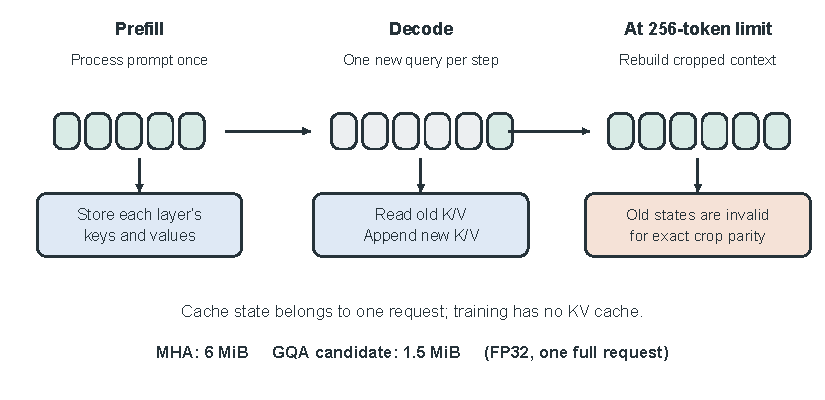
\includegraphics[width=\linewidth]{cache.pdf}
\caption{The inference context policy. Cached decoding accelerates growth within the trained window. Once the fixed 256-token context is full, the implementation rebuilds from the cropped text to preserve equivalence with uncached generation. It does not silently substitute a longer-history model.}
\label{fig:cache}
\end{figure}

This crop policy is consequential. Learned positions change after a crop; even with RoPE, deeper retained states still contain information from evicted tokens. Simply deleting the oldest cache entries would not reproduce a fresh forward pass over the cropped window. The implementation therefore rebuilds at overflow. On the learned-position checkpoint, caching accelerated a 32-token prompt plus 64 generated tokens by 1.157$\times$, but a 248-token prompt plus 64 outputs by only 1.0165$\times$. A single-token decode after 128 prior positions improved from 3.31775 to 2.57654 ms. These are synchronized local model timings, not HTTP throughput and not a new benchmark of the later RoPE checkpoint.

\subsection{O17: BF16 inference on the RoPE checkpoint}
BF16 training saved time, but inference has different shapes and memory demands. I compared FP32 and BF16 autocast on the identified 256-context RoPE export without changing its FP32 weights. Each timing condition used three warmup pairs followed by 20 interleaved pairs. Both precisions scored the same familiar-validation targets; a separate probability comparison used 10,240 targets.

Validation loss changed from 4.08818384 to 4.08820787, a +0.00002403-nat difference. Mean $D_{\mathrm{KL}}(P_{\mathrm{FP32}}\Vert P_{\mathrm{BF16}})$ was 0.00007131 and top-1 agreement was 98.94\%. Cached and uncached predictions were compared within each precision at 20 real positions spanning context overflow. Maximum relative root-mean-square logit error was $3.18\times10^{-7}$ for FP32 and 0.004964 for BF16; the checked greedy choices agreed. These results passed the prespecified numerical tolerances.

The performance result was less favorable. For 32 prompt tokens and 64 generated tokens, median time increased from 0.193243 to 0.229446 seconds (+18.73\%). For a near-full 248-token prompt, it decreased from 0.383007 to 0.370971 seconds (-3.14\%). The persistent full-window cache shrank from 6 to 3 MiB, but sampled live allocation after 129 cache positions barely changed: 113,640,448 versus 113,637,376 bytes. This did not meet either acceptance route: at least 5\% speed improvement in both prompt conditions, or at least 20\% less sampled live memory with at most 5\% slower generation. I did not run the optional 20-sample text audit after this performance failure. FP32 inference remains the choice for this checkpoint. These are MPS measurements, not a production-CPU BF16 result.

\subsection{What generated text does and does not show}
\label{sec:generation-audit}
The common generation audit uses five prompts, four sampling seeds, temperature 0.8, top-$k$ 40, and 256 new tokens per continuation. Prompts include the hero's name, Bakai, a dialogue opening, and an action opening. The repository's generation-audit records retain the complete prompt/seed list. Temperature rescales logits before softmax; top-$k$ restricts the candidates. Generation then samples one token, appends it, and repeats. The model has no supervised fine-tuning, preference optimization, reinforcement learning from human feedback, retrieval, or external language model.

The saved continuations contain epic-associated names and short action or dialogue fragments. The model also changes actors abruptly, forms malformed endings, repeats titles, and fails to maintain long narrative state. These qualitative observations come from reading the saved outputs; I have no blinded native-speaker fluency or coherence study. The repeated-trigram ratio counts word-trigram occurrences beyond their first occurrence, divided by all word-trigram occurrences. The reported mean averages this ratio across 20 continuations. A sample with zero repeated trigrams can still wander semantically.

The copying audit itself required correction. The old matcher normalized generated words but searched an unnormalized source string, missing matches across punctuation and line breaks. Symmetric word normalization changed the frozen 27M audit's maximum matching span from seven to nine words. Nine of its 20 per-sample counts changed. A bounded real-source positive control then matched all 142 words. I re-audited saved outputs rather than regenerating them under new randomness. Current copying results describe case-folded, punctuation-insensitive whole-word spans, \emph{not} exact byte copying. An observed maximum of eleven words in 20 RoPE samples cannot establish an absence of memorization elsewhere.

\subsection{The delivered model is an identified artifact}
The native RoPE export is 107,157,586 bytes, with a recorded SHA-256 distinct from its optimizer-bearing research checkpoint. The release check reloaded it through the actual model path, reproduced logits, and verified greedy cache parity across overflow; maximum recorded cache logit difference was $6.20\times10^{-6}$. The original model artifacts were preserved for rollback.

Serving uses FP32 with bounded generation: one request at a time, 16--128 new tokens, temperature 0.5--1.2, and top-$k$ 1--100. The public website calls an authenticated private model service through its own rate-limited route; it does not send users' requests to another language model. The release record includes a successful public generation check. That proves a working path at release time, not sustained concurrency, an inference service-level agreement, or a new quality evaluation.

\section{Discussion and limitations}
\label{sec:discussion}
\paragraph{Scope of the findings.}
Within the original Manas-only recipe, more capacity improved prediction, mixed precision improved training cost, and RoPE improved held-out loss. Increasing context, changing the activation, reducing vocabulary, or sharing KV heads did not automatically improve the delivered model. The later corpus expansion improved a different book score but failed the familiar-domain floor, while BF16 inference failed its performance gate. These outcomes support retaining changes that helped under the measured conditions and stated quality constraints.

\paragraph{Stopping rules should match the question.}
Equivalence optimizations can fail on correctness or cost without a full training run. Architectural changes deserve a quality check if a modest cost increase could buy a useful gain. RoPE demonstrates the opportunity cost of the original speed-first filter. RMSNorm demonstrates the complementary limit: a flat early comparison can justify saving resources, but cannot prove that the final ordering would remain unchanged. Reopening a rule must be recorded rather than quietly rewriting the old decision.

\paragraph{Measurement definitions can change a conclusion.}
Scheduled validation and additional validation use different samples. Exact-byte BPB, timing, memory, and copying measurements also require explicit denominators and definitions. Comparing mismatched measurements can create an apparent improvement even when the model is unchanged.

\paragraph{Data and statistical limitations.}
The deployed model still uses one edition of one epic. The O15 research arm adds three volumes, and O14 supplies a separate book for validation and a different narrator for test. These are limited source groups, not a broad Kyrgyz benchmark. Formulaic language, related editions, residual OCR errors, formatting differences, and historical tokenizer exposure constrain interpretation. The final Mamay score belongs only to the retained model. There is no general Kyrgyz task suite, multi-seed confidence interval, hyperparameter sweep for every candidate, or external baseline study. Validation was repeatedly consulted, and the historical test suffix had already been evaluated in earlier phases. The reported gains are evidence for this experimental sequence, not unbiased estimates on an unseen population of tasks.

\paragraph{Hardware and reproducibility limitations.}
MPS timings were measured on a shared 16 GB M5 host. Sequential full runs can experience different background load and temperature. Interleaved short comparisons reduce, but do not eliminate, this concern. Compiler and RNG observations are tied to the inspected runtime. Saved data, hashes, configurations, and curves enable auditing; exact future floating-point trajectories across platforms are not promised. Raw licensed corpora and weight files are not committed to Git, so public source access alone is not a claim that all artifacts are publicly downloadable.

\paragraph{Use limitations and next experiments.}
Tiny Manas is unsuitable as a general assistant, a factual reference for the epic, or a reliable Kyrgyz writing tool. A small prediction-score improvement does not establish cultural or linguistic ``understanding.'' O14/O15 show why text preparation and evaluation design need attention before attributing a gain to diversity. The remaining questions include representation-consistent data comparisons, adequate matched training budgets, repeated seeds, and human review of coherence. This follow-up did not introduce quantization, request batching, a new attention backend, a runtime upgrade, or supervised fine-tuning.

\section{Conclusion}
I progressed from a fixed-batch learning check to a versioned 26.78M-parameter RoPE decoder that generates Manas-like text. The September 5 follow-up retained its frozen 32k tokenizer, BF16 training, and FP32 cached inference within 256 tokens. Additional books improved the new-book score but violated the familiar-domain floor; the longer-context pilot stopped without consistent primary improvement; BF16 inference was numerically close but too costly for short generation. The new holdouts also exposed weak source transfer in the retained model. Saved configurations, curves, negative outcomes, and artifact hashes link these conclusions to the actual runs. They remain findings about these corpora and budgets, with limited narrative coherence and no general Kyrgyz-assistant claim.

\begin{thebibliography}{14}
\small
\raggedright
\bibitem{attention} Ashish Vaswani, Noam Shazeer, Niki Parmar, Jakob Uszkoreit, Llion Jones, Aidan N. Gomez, Łukasz Kaiser, and Illia Polosukhin. \emph{Attention Is All You Need}. NeurIPS, 2017. \href{https://arxiv.org/abs/1706.03762}{arXiv:1706.03762}.
\bibitem{gpt2} Alec Radford, Jeffrey Wu, Rewon Child, David Luan, Dario Amodei, and Ilya Sutskever. \emph{Language Models are Unsupervised Multitask Learners}. OpenAI technical report, 2019. \href{https://cdn.openai.com/better-language-models/language_models_are_unsupervised_multitask_learners.pdf}{Original report}.
\bibitem{dropout} Nitish Srivastava, Geoffrey Hinton, Alex Krizhevsky, Ilya Sutskever, and Ruslan Salakhutdinov. \emph{Dropout: A Simple Way to Prevent Neural Networks from Overfitting}. Journal of Machine Learning Research, 15:1929--1958, 2014. \href{https://jmlr.org/papers/v15/srivastava14a.html}{JMLR article}.
\bibitem{layernorm} Jimmy Lei Ba, Jamie Ryan Kiros, and Geoffrey E. Hinton. \emph{Layer Normalization}. arXiv preprint, 2016. \href{https://arxiv.org/abs/1607.06450}{arXiv:1607.06450}.
\bibitem{adamw} Ilya Loshchilov and Frank Hutter. \emph{Decoupled Weight Decay Regularization}. ICLR, 2019. \href{https://arxiv.org/abs/1711.05101}{arXiv:1711.05101}.
\bibitem{checkpoint} Tianqi Chen, Bing Xu, Chiyuan Zhang, and Carlos Guestrin. \emph{Training Deep Nets with Sublinear Memory Cost}. arXiv preprint, 2016. \href{https://arxiv.org/abs/1604.06174}{arXiv:1604.06174}.
\bibitem{rope} Jianlin Su, Yu Lu, Shengfeng Pan, Ahmed Murtadha, Bo Wen, and Yunfeng Liu. \emph{RoFormer: Enhanced Transformer with Rotary Position Embedding}. arXiv preprint, 2023 (version 5; first posted 2021). \href{https://arxiv.org/abs/2104.09864v5}{arXiv:2104.09864v5}.
\bibitem{rmsnorm} Biao Zhang and Rico Sennrich. \emph{Root Mean Square Layer Normalization}. NeurIPS, 2019. \href{https://arxiv.org/abs/1910.07467}{arXiv:1910.07467}.
\bibitem{swiglu} Noam Shazeer. \emph{GLU Variants Improve Transformer}. arXiv preprint, 2020. \href{https://arxiv.org/abs/2002.05202}{arXiv:2002.05202}.
\bibitem{gqa} Joshua Ainslie, James Lee-Thorp, Michiel de Jong, Yury Zemlyanskiy, Federico Lebrón, and Sumit Sanghai. \emph{GQA: Training Generalized Multi-Query Transformer Models from Multi-Head Checkpoints}. EMNLP, 2023. \href{https://arxiv.org/abs/2305.13245}{arXiv:2305.13245}.
\bibitem{cce} Erik Wijmans, Brody Huval, Alexander Hertzberg, Vladlen Koltun, and Philipp Krähenbühl. \emph{Cut Your Losses in Large-Vocabulary Language Models}. ICLR, 2025. \href{https://arxiv.org/abs/2411.09009}{arXiv:2411.09009}.
\bibitem{hyperband} Lisha Li, Kevin Jamieson, Giulia DeSalvo, Afshin Rostamizadeh, and Ameet Talwalkar. \emph{Hyperband: A Novel Bandit-Based Approach to Hyperparameter Optimization}. Journal of Machine Learning Research, 18(185):1--52, 2018. \href{https://jmlr.org/papers/v18/16-558.html}{JMLR article}.
\bibitem{nanogpt} Andrej Karpathy. \emph{nanoGPT}. Software repository, accessed September 4, 2026. \href{https://github.com/karpathy/nanoGPT}{github.com/karpathy/nanoGPT}. Consulted as an implementation reference; Tiny Manas is a separate implementation.
\bibitem{bizdin} Bizdin. \emph{Manas collection: editions attributed to Sagymbay Orozbakov and Jusup Mamay}. Digital source catalogue, accessed September 5, 2026. \href{https://new.bizdin.kg/knigi/category/manas}{new.bizdin.kg/knigi/category/manas}. Exact PDFs, verse-page ranges, and SHA-256 locks are identified in the O14 experiment record.
\end{thebibliography}

\end{document}
